\chapter{C programming}
The C is the most powerful language and also can be considered as the language nearest to Assembly language. Its power is the speed of execution and the easy interpretation of the memory.\\
C can be considered very important in Computer Networks because it doesn't hide the use of system calls. Other languages made the same thing, but hiding all the needs and evolution of Computer Network systems.

\section{Organization of data}\label{littleBig}
Data are stored in the memory in two possible ways, related to the order of bytes that compose it. There are two main ways, called Big Endian and Little Endian.
\begin{center}
\begin{tabular}{c}
\begin{lstlisting}[linewidth=30pt, basicstyle=\footnotesize\sffamily,]
int i;
\end{lstlisting}
\end{tabular}
\end{center}

\begin{figure}[h]
\centering
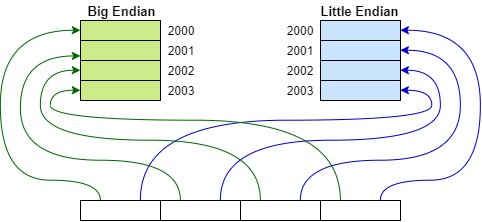
\includegraphics[scale=0.68]{Images/Programming/endians}
\caption{\footnotesize{Little Endian and Big Endian.}}
\end{figure}

The size of \textbf{int, float, char, ...} types
depends on the architecture used. The max size of possible types depends on the architecture (E.g. in 64bits architecture, in one istruction, 8 bytes can be written and read in parallel).

\begin{table}[h]
\centering
\begin{tabular}{|c|c|}
\hline
\textbf{signed}&{unsigned}\\
\hline
{int8\_t}&{uint8\_t}\\
{int16\_t}&{uint16\_t}\\
{int32\_t}&{uint32\_t}\\
{int64\_t}&{uint64\_t}\\
\hline
\end{tabular}\caption{<stdint.h>}
\end{table}
\vspace{4cm}
\section{Struct organization of memory}
The size of a structure depends on the order of fields and the architecture. This is caused by alignment that depends on the number of memory banks, number of bytes read in parallel. For example the size is 4 bytes for 32 bits architecture, composed by 4 banks (Figure \ref{parallel}).
\begin{center}
\begin{tabular}{c}
\begin{lstlisting}[linewidth=200pt, basicstyle=\footnotesize\sffamily,]
struct example1        struct example2
{                      {
	char c;	               int x;
	int x;	               char c;
}                      }
\end{lstlisting}
\end{tabular}
\end{center}

\begin{figure}[h]
\centering
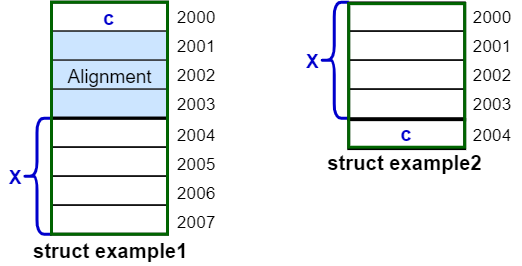
\includegraphics[scale=0.5]{Images/Programming/struct}
\end{figure}

\begin{figure}[h]
\centering
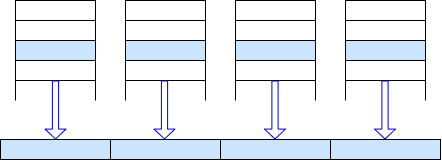
\includegraphics[scale=0.68]{Images/Programming/parallel_reading}
\caption{\footnotesize{Parallel reading in one istruction in 32 bits architecture.}}\label{parallel}
\end{figure}

\vspace{3cm}
\section{Structure of C program}
The program stores the variable in different section (Figure \ref{program}):
\begin{itemize}
\item{\textbf{Static area}\\
where global variables and static library are stored, it's initialized immediately at the creation of the program. Inside this area, a variable doesn't need to be initialized by the programmer because it's done automatically at the creation of the program with all zeroes.}
\item{\textbf{Stack}\\
allocation of variables, return and parameters of functions}
\item{\textbf{Heap}\\
dinamic allocation }
\end{itemize}

\begin{figure}[h]
\centering
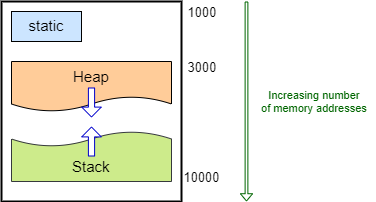
\includegraphics[scale=0.68]{Images/Programming/program}
\caption{\footnotesize{Structure of the program.}}\label{program}
\end{figure}